\documentclass[12pt, letterpaper]{article}

%-------Packages---------
\usepackage{amssymb,amsfonts}
\usepackage{mathptmx}
\usepackage{amsthm}
\usepackage{graphicx}
\usepackage[all,arc]{xy}
\usepackage[colorlinks=true, allcolors=blue]{hyperref}
\usepackage{enumerate}
\usepackage{bbm}
\usepackage{dsfont}
\usepackage{mathrsfs}
\usepackage{tikz-cd}
\usepackage{setspace}
\usepackage{import}
\usepackage[utf8]{inputenc}
\usepackage{hyperref}
\usepackage{tikz}
\usepackage{float}
\usepackage{mdframed}
\usepackage[nocheck]{fancyhdr}
\usepackage[nointegrals]{wasysym}

\usepackage[left=1in,top=1in,right=1in,bottom=1in]{geometry}

\usepackage{mathtools}
\usepackage{setspace}
\usepackage{cleveref}
\usepackage{multicol}
\usepackage{mathpazo}

\usepackage{algorithm}
\usepackage[noend]{algpseudocode}
\usetikzlibrary{positioning}

\newcounter{problem}

% Define a new command for problems
\newcommand{\q}{
    \newpage % Start a new page
    \stepcounter{problem} % Increment problem counter
    \subsection*{Problem \arabic{problem}} % Display the problem counter
}
\newcommand{\C}{\mathbb{C}}
\newcommand{\R}{\mathbb{R}}
\newcommand{\Q}{\mathbb{Q}}
\newcommand{\Z}{\mathbb{Z}}
\newcommand{\N}{\mathbb{N}}
\renewcommand{\P}{\mathbb{P}}
\newcommand{\F}{\mathbb{F}}
\newcommand{\contr}{\Rightarrow \Leftarrow}
\newcommand{\HRule}[1]{\rule{\linewidth}{#1}}
\newcommand{\s}{\(\,\)}
\renewcommand{\t}[1]{\text{#1}}
\newcommand{\ang}[1]{\left\langle #1 \right\rangle}

% Meta data
\setstretch{1.2}

\begin{document}
\setlength{\parindent}{0pt}
\pagestyle{fancy}
\fancyhf{}
\fancyhead[LOE]{\slshape{\textbf{Vincent Ferrara}}}
\fancyhead[ROE]{\thepage}

\q
\begin{enumerate}[i.]\addtocounter{enumi}{4}
    \item Consider $(x^2-y,x^3-z)=A$. We can see that $A \subset \ker$ since $f(x^2-y)=t^2-t^2=0$ and $f(x^3-z)=0$
    
    Consider $C[x,y,z] \diagup A$. Let $g \in \ker$, now in the quotient ring we can rewrite $g$ s.t.:
    \[y=x^2, z=x^3\]
    This means this new polynomial is equivalent to some $g'(x)=g(x,x^2,x^3) \in \C[x]$.

    Since we know that $g(t,t^2,t^3)=0$ this implies that $g'(t)=g(t,t^2,t^3)=0$ for all $t \in \C$. Now since $g'$ is a single variable and is zero for all $t$ this implies it is the zero polynomial. Thus, this implies it is in $A$. Thus $\ker=A$
\end{enumerate}

\q
\begin{enumerate}[(a)]\addtocounter{enumi}{1}
    \item From $(a)$ we know that $I^e \subseteq I^{ec}$. Thus, we can let $I=I^e$ thus $I^{e} \subseteq I^{ece}$
    
    Let $x \in I^{ece} \implies x=\sum_{i = 1}^n r_i x_i$ s.t. $r_i \in B$ and $x_i \in \phi(I^{ec})$. This implies there is a $a_i \in I^{ec}$ s.t. $x_i=\phi(a_i)$.
    \[ x=\sum_{i = 1}^n r_i\phi(a_i)\]
    Since $a_i \in I^{ec}=\phi^{-1}(I^e)$ this means that $\phi(a_i) \in I^e$ this implies that $x \in I^e$ since ideals are closed under multiplication from any element and addition withing the ideal. Thus $I^e = I^{ece}$

    From $(a)$ we know that $J^{ec} \subseteq J$. Thus, we can let $J=J^c \implies J^{cec} \subseteq J^c$

    Let $x \in J^{cec} \implies x \in \phi^{-1}(J^{ce}) \implies \phi(x) \in J^{ce}$. Thus, $\phi(x)$ is in the form:
    \[\phi(x)=\sum_{i=1}^{n}r_ix_i\]
    s.t. $r_i \in B$ and $x_i \in \phi(J^c) \implies \exists a_i \in J^c=\phi^{-1}(J)$ s.t. $\phi(a_i)=x_i \implies x_i \in J \implies \varphi(x) \in J \implies x \in J^c$

    Thus, $J^{cec}=J^c$.

    \item Let $q$ be a prime ideal in $B$. The consider:
    \[q^c=\phi^{-1}(q)=\{a \in A \mid \phi(a) \in q\}\]
    Let $a,b \in q^c$ this means that $\phi(ab)=\phi(a)\phi(b) \in q$. This means that:
    \[\phi(a) \in q \quad \t{ or } \quad \phi(b) \in q\]
    This implies that 
    \[a \in q^c \quad \t{ or } \quad b \in q^c\]

    Consider the natural injective map $\phi:\Z \to \Q$. Consider the $(0) \subseteq \Q$. This is maximal since $\Q$ is a field, so there is only ideals $(0),\Q$

    Consider $(0)^c=\{a \in \Z \mid \phi(a)=0\}=(0)$ since $\phi$ is injective. However, $(0) \subset (2)$ is not maximal in $\Z$.
\end{enumerate}

\q
Consider $\varphi:\Z[i] \diagup (5) \to \F_5 \times \F_5$ s.t. $\varphi(a+bi)=(a-2b, a+2b) \mod 5$

Injective:

Let $a+bi \in \ker{\varphi}$ then $\varphi(a+bi)=(0,0)$. This means that $a=2b$ and $a=-2b$ this implies $4b=0$ thus multiply by 4, and we get $b=0$ thus $a=0$. Thus, injective.

Surjective:

Let $(c,d) \in \F_5 \times \F_5$. Let $a=3(c+d) \mod 5$ and let $b=4(d-c) \mod 5$. Thus consider $\varphi(a,b)=(a-2b,a+2b) \mod 5=(3c+3d-8d+8c,3c+3d+8d-8c) \mod 5=(c,d) \mod 5$ Thus, surjective.

Homomorphism:

$\varphi(1)=(1,1)$

Let $a+bi,c+di \in \Z[i] \diagup (5)$

$\varphi(a+c+(b+d)i)=(a+c-2b-2d,a+c+2b+2d)=(a-2b,a+2b)+(c-2d,c+2d)=\varphi(a+bi)+\varphi(c+di)$\\


$\varphi((a+bi)(c+di))\varphi(ac+adi+cbi-bd)=\varphi(ac-bd+(ad+cb)i)=(ac+4bd-2ad-2cb,ac+4bd+2ad+2cb)=((a-2b)(c-2d),(a+2b)(c+2d))=\varphi(a+bi)\varphi(c+di)$

Thus $\Z[i] \diagup \F_5 \times \F_5$

Proven in HW1 we know that ideals of $\F_5 \times \F_5$ are of the form ideals in $I \times J$ s.t. $I$ is an ideal in $\F_5$. Thus, since $\F_5$ is a field we know the only ideals are $(0),\F_5$. Thus, we have 4 ideals:
\begin{itemize}
    \item $(0) \times (0)$
    \item $\F_5 \times \F_5$
    \item $\F_5 \times (0)$
    \item $(0) \times \F_5$
\end{itemize}

Mapping these back to $\Z[i] \diagup (5)$ we get $(0) \times (0) \cong (0),(0) \times \F_5 \cong (2-i),\F_5 \times (0) \cong (2+i), \F_5 \times \F_5 \cong (1)$.

$(0)$ is not prime since $(2-i)(2+i)=5=0$. Thus, not maximal.

$(1)$ is not prime and maximal by definition.

$(0) \times \F_5$ is maximal since if we add anything to the $(0)$ part since $\F_5$ is a field everything is a unit except zero, so we would get the whole ring. Thus, $(2-i),(2+i)$ are maximal thus prime.

\q

\begin{enumerate}[(a)]
    \item \begin{enumerate}[iv.]
        \item Consider $7=(4x+5)(4x-5)-8(2x^2-4)$. Thus, $7 \in (2x^2-4,4x-5)$.
        \begin{align*}
            4x-5 &\equiv 0 \pmod{7}\\
            4x &\equiv 5 \pmod{7}\\
            x &\equiv 3 \pmod{7}
        \end{align*}
        Thus $(2x^2-4,4x-5)=(x-3,7)$ since $4(x-3)+7=4x-5$ and $(2x+6)(x-3)+14=2x^2-4$. Thus:
        \[\dfrac{\Z[x]\diagup(x-3)}{(x-3,7) \diagup (x-3)} \cong \Z \diagup (7) \cong \Z \diagup 7\Z\]
    \end{enumerate}
    \item Assume for contradiction they are isomorphic. 
    
    This implies that $\Z[x] \diagup (x^2+7,2) \cong \Z[x] \diagup (2x^2+7,2)$. 
    
    However, this implies that $\Z[x] \diagup (2x^2+7,2)=\Z[x] \diagup (0+7,2) = (0)$ since $7-2(3)=1$. 
    
    However, $\Z[x] \diagup (x^2+7,2) = \Z[x] \diagup (x^2+1,2) \cong \F_2[x] \diagup(x^2+1)=\{0,1,x,1+x\} \neq (0)$.

    \item If $p=2$:
    \[\Z[i]\diagup (2) \cong \dfrac{\Z[x] \diagup (x^2+1)}{(2)} \cong \dfrac{\Z[x] \diagup (x^2+1)}{(2,x^2+1) \diagup (x^2+1)} \cong \Z[x] \diagup (2,x^2+1)\]
    \[\Z[x] \diagup (2,x^2+1) \cong \dfrac{\Z[x] \diagup (2)}{(2,x^2+1) \diagup (2)} \cong \F_2[x] \diagup (x^2+1)=F_2[x] \diagup (x-1)^2\]

    Let \begin{align*}
        R_1 &= \mathbb{F}_2[x]/(x-1)^2, \\
        R_2 &= \mathbb{F}_2[x]/(x^2).
    \end{align*}
    
    Define a map:
    \[
        \varphi: \F_2[x] \to \F_2[x]
    \]
    by:
    \[
        \varphi(f(x))=f(x+1)
    \]
    This is an automorphism.
    Define a map:
    \[
        \psi: \F_2[x]\diagup((x-1)^2) \to \F_2[x]\diagup(x^2)
    \]
    by:
    \[
        \psi(a+((x-1)^2))=\varphi(a)+\varphi((x-1)^2)=\varphi(a)+(x^2)
    \]

    Well-Defined:

    Assume that \(r + ((x-1)^2) = s + ((x-1)^2)\) for some \(r, s \in \F_2[x]\). Then
    \[
    r - s \in ((x-1)^2).
    \]
    Since \(\varphi\) is a ring homomorphism, we have
    \[
    \varphi(r - s) = \varphi(r) - \varphi(s) \in (x^2).
    \]
    Thus,
    \[
    \varphi(r) + (x^2) = \varphi(s) + (x^2),
    \]
    which shows that \(\psi(r + ((x-1)^2)) = \psi(s + ((x-1)^2))\). Therefore, the map is well-defined.

    Homomorphism:

    For \(r, s \in \F_2[x]\), we have
    \[
    \psi((r+s) + ((x-1)^2)) = \varphi(r+s) + (x^2) = (\varphi(r) + \varphi(s)) + (x^2),
    \]
    \[
    \psi(rs + ((x-1)^2)) = \varphi(rs) + (x^2) = \varphi(r)\varphi(s) + (x^2),
    \]

    Bijective

    Since \(\varphi\) is an automorphism of \(\F_2[x]\), it is bijective. Its inverse \(\varphi^{-1}\) is also an automorphism. The inverse of \(\psi\) is given by
    \[
    \psi^{-1}: R/(x^2) \to R/((x-1)^2), \quad \psi^{-1}(r + (x^2)) = \varphi^{-1}(r) + ((x-1)^2).
    \]
    Thus, \(\psi\) is bijective.

    \textbf{Conclusion.}

    Since \(\psi\) is a well-defined ring homomorphism that is bijective, we conclude that
    \[
    \F_2[x]/((x-1)^2) \cong \F_2[x]/(x^2).
    \]
    
    Let $p$ be odd and assume there exists a $a \in \Z$ s.t. $a^2 \equiv -1 \pmod{p}$

    \[\Z[i]\diagup (p) \cong \dfrac{\Z[x] \diagup (x^2+1)}{(p)} \cong \dfrac{\Z[x] \diagup (x^2+1)}{(p,x^2+1) \diagup (x^2+1)} \cong \Z[x] \diagup (p,x^2+1)\]
    \[\Z[x] \diagup (p,x^2+1) \cong \dfrac{\Z[x] \diagup (p)}{(p,x^2+1) \diagup (p)} \cong \F_p[x] \diagup (x^2+1) \cong \F_p[x] \diagup (x-a)(x+a)\]

    Thus, since $x-a-x-a=-2a$. Since $p$ is odd this implies that $-2a \neq 0$. Since we are in $\F_p$ we know we can find an inverse for $-2a$ let that be $b$. Thus, $b(x-a)+b(x+a)=b(-2a)=1$ Thus by the CRT:
    \[\F_p[x] \diagup (x-a)(x+a) \cong \F_p[x] \diagup (x-a) \times \F_p[x] \diagup (x+a)\]

    Define $\varphi: \F_p[x] \to \F_p$ s.t. $f(x) \mapsto f(a)$

    Homomorphism:

    \begin{itemize}
        \item $\varphi(f(x)+g(x))=f(a)+g(a)=\varphi(f(x))+\varphi(g(x))$
        \item $\varphi(f(x)g(x))=f(a)g(a)=\varphi(f(x))\varphi(g(x))$
        \item $\varphi(1)=1$
    \end{itemize}

    This is clearly surjective since $f(k)=k$ for $k \in \F_p$

    The kernel is also all polynomial's with a root of $a$ thus this is the set divisible by $x-a$ which his $(x-a)$

    Thus by the first isomorphism theorem $\F_p[x] \diagup (x-a) \cong \F_p$ do the same for $\F_p[x] \diagup (x+a) \cong \F_p$

    \[\F_p[x] \diagup (x-a) \times \F_p[x] \diagup (x+a) \cong \F_p \times \F_p\]

    Let $p$ be odd s.t. there is no integer s.t. $x^2 = -1 \pmod {p}$

    Ok do the same thing as above, and we get to $\Z[i] \diagup (p) \cong \F_p[x] \diagup (x^2+1)$. Since there is no integer s.t. $x^2 = -1$ this implies that $(x^2+1)$ is irreducible in $\F_p[x]$. Thus proven in class since this is not zero we know that $(x^2+1)$ is prime and maximal. Thus proven in class since $(x^2+1)$ is maximal this implies that $F_p[x] \diagup (x^2+1)$ is a field.

    Now for the size. Since we have the relation $x^2=-1$ this implies that we can write every polynomial in $\F_p[x]$ as:
    \[a+bx, \quad a,b \in \F_p\]

    The reason is if we have a term $cx^n$ s.t. $c \in \F_p$ and $n > 1$. We can use the division algorithm and get $n=2q+r$ s.t. $q \in \N$ and $r \in \{0,1\}$

    Thus $cx^n=c(-1)^qx^r$

    Thus, since $a,b$ are chosen independently in $\F_p$ we get $p$ choices for $a$ and $p$ for $b$ thus we get $p^2$ elements.

    \item \[
            \mathbb{Z}[\omega]/(p) \cong
            \begin{cases}
            \mathbb{F}_3[t]/(t^2), & \text{if } p = 3,\\
            \mathbb{F}_p \times \mathbb{F}_p, & \text{if $p\neq3$ and } \exists a \in \Z \text{ s.t. } a^3=1,a\neq1 \pmod{p},\\
            \text{a field with } p^2 \text{ elements}, & \text{if $p\neq3$ and there is not an integer as described above}.
            \end{cases}
            \]
    
    Define $\varphi: \Z[\omega] \to \Z[x]$ s.t. $\varphi(f(x))=f(\omega)$ This is the same proof as in (c). This is a surjective homomorphism with kernel $(x^2+x+1)$ thus $\Z[\omega] \cong \Z[x] \diagup (x^2+x+1)$

    If $p=3$

    \[\Z[\omega]\diagup (3) \cong \dfrac{\Z[x] \diagup (x^2+x+1)}{(3)} \cong \dfrac{\Z[x] \diagup (x^2+x+1)}{(3,x^2+x+1) \diagup (x^2+x+1)} \cong \Z[x] \diagup (3,x^2+x+1)\]
    \[\Z[x] \diagup (3,x^2+x+1) \cong \dfrac{\Z[x] \diagup (3)}{(3,x^2+x+1) \diagup (3)} \cong \F_3[x] \diagup (x^2+x+1)=\F_3[x] \diagup (x-1)^2\]

    Use a similar proof for the $p=2$ case in part (c) to show that $\F_3[x] \diagup (x-1)^2 \cong \F_2[x] \diagup (x^2)$

    If $p \neq 3$ and there is an $a \in \Z \setminus \{1\}$ s.t. $a^3 = 1,a\neq 1 \pmod{p}$.

    Then again we get $\Z[\omega] \diagup (p) \cong \F_p[x] \diagup (x^2+x+1)$. Since $a^3 = 1 \implies a^3-1=0 \implies (a-1)(a^2+a+1)=0$ and since $a \neq 1$ we know that $a-1$ is not zero thus we can cancel it since we are in a field, and we get that $(a^2+a+1)=0$. Now consider $(x-a)(x+a+1)=x^2+ax+x-ax-a^2-a$. Since $a^2+a=-1$, $x^2+ax+x-ax-a^2-a=x^2+x+1$.

    Since $x+a+1-x+a=2a+1$. We get that these are coprime since we can get to one since we are in a field. Thus by CRT

    \[\F_p[x] \diagup (x-a)(x+a+1) \cong \F_p[x] \diagup (x-a) \times \F_p[x] \diagup (x+a+1)\]

    Now do a similar proof from part (c) and we get $\cong \F_p \times \F_p$

    If $p \neq 3$ and we do not have that property then this means that $(x^2+x+1)$ is irreducible thus we do the same proof to show that $\Z[\omega] \diagup (p)$ is a field with $p^2$ elements.
 \end{enumerate}

 \q

 \begin{enumerate}[(a)]
    \item Let $E=\{0\}$. Since every ideal has $0$ this implies that $V(0)=\text{Spec}(A)$. Thus, $X$ is closed.
    
    Let $E=\{1\}$. Since if an ideal contains $1$ then it is the whole ring, and since prime ideals are not the whole ring we get that $V(1)=\emptyset$. Thus, $\emptyset$ is closed.

    Let $\{E_i\}_{i\in I}$ be a collection of subsets of $A$. Consider:
    \[E=\bigcap_{i \in I} V(E_i)\]
    By definition a prime ideal $p$ belongs to $V(E_i) \iff E_i \subseteq p$. Thus if $p \in E$ then $E_i \subset p$ for all $i \in I$. Thus:

    \[\left( \bigcup_{i \in I} E_i \right) \subset p\]
    Thus:
    \[p \in V\left( \bigcup_{i \in I} E_i \right)=B\]

    Let $p \in B$ thus
    \[\left( \bigcup_{i \in I} E_i \right) \subset p\]
    Thus we know that $E_i \subseteq p$ for all $i \in I$. Thus, we know that $p \in E$.

    Thus, $E=B$, $E$ is closed since $B$ is closed.

    Consider $V(E) \cup V(F)$ for $E,F \subseteq A$. Consider $EF$ the ideal generated by products of $ef$ s.t. $e \in E$ and $f \in F$

    Let $p \in V(E) \cup V(F)$. Then either $E \subset p$ or $F \subset p$. In either case, if $e \in E$ and $f \in F$, then either $e \in p$ or $f \in p$. Since $p$ is a prime ideal, it follows that $ef \in p$. Thus, every element of $EF$ is in $p$, and so $p \in V(EF)$.

    Let $p \in V(EF)$ thus $EF \subset p$. Assume for contradiction that $p \notin V(E)$ and $p \notin V(F)$. Then there exists $e \in E$ and $f \in F$ s.t. $e \notin e$ and $f \notin p$. But since $p$ is prime, this means that $ef \notin p$. This is a contradiction. Thus either $E \subset p$ or $F \subset p$ thus $p \in V(E) \cup V(F)$.

    Thus, $V(E)$ satisfy the axioms of closed sets.

    \setcounter{enumi}{4}\item 
    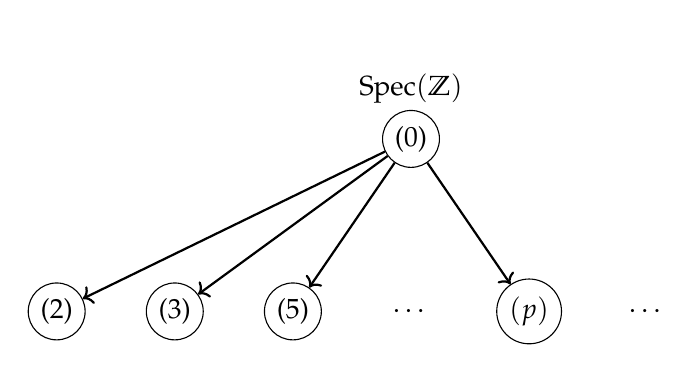
\begin{tikzpicture}[node distance=1.5cm, auto, every node/.style={draw, circle, inner sep=2pt}]
        % Generic point (0)
        \node (zero) {(0)};
        
        % Closed points for a few primes
        \node (dots) [below =of zero,draw=none] {$\dots$};
        \node (p) [right of= dots] {$(p)$};
        \node (dots2) [right of= p,draw=none] {$\dots$};

        \node (p5) [left of= dots] {(5)};
        \node (p3) [left of= p5] {(3)};
        \node (p2) [left of= p3] {(2)};
        
        % Arrows indicating specialization: (0) specializes to every maximal ideal.
        \draw[->, thick] (zero) -- (p2);
        \draw[->, thick] (zero) -- (p3);
        \draw[->, thick] (zero) -- (p5);
        \draw[->, thick] (zero) -- (p);

        \node[above=-0.5 of zero, align=center, draw=none] 
        {\(\operatorname{Spec}(\mathbb{Z})\)};
      \end{tikzpicture}

      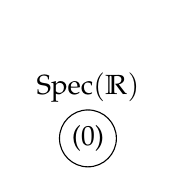
\begin{tikzpicture}[node distance=1.5cm, auto, every node/.style={draw, circle, inner sep=2pt}]
        \node (zero) {(0)};
        \node[above=-0.5 of zero, align=center, draw=none] 
        {\(\operatorname{Spec}(\mathbb{R})\)};
      \end{tikzpicture}

      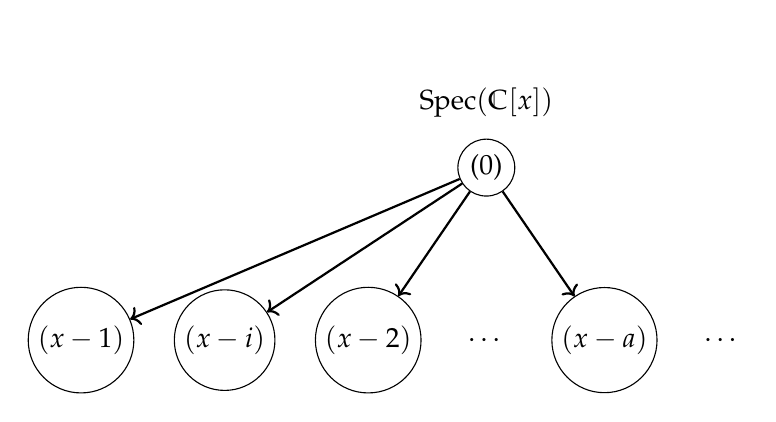
\begin{tikzpicture}[node distance=1.5cm, auto, every node/.style={draw, circle, inner sep=2pt}]
        % Generic point (0)
        \node (zero) {(0)};
        
        % Closed points for a few primes
        \node (dots) [below =of zero, draw=none] {$\dots$};
        \node (p) [right of= dots] {$(x-a)$};
        \node (dots2) [right of= p, draw=none] {$\dots$};

        \node (p5) [left of= dots] {$(x-2)$};
        \node (p3) [left =0.5of p5] {$(x-i)$};
        \node (p2) [left =0.5of p3] {$(x-1)$};
        
        % Arrows indicating specialization: (0) specializes to every maximal ideal.
        \draw[->, thick] (zero) -- (p2);
        \draw[->, thick] (zero) -- (p3);
        \draw[->, thick] (zero) -- (p5);
        \draw[->, thick] (zero) -- (p);

        \node[above=-0.5 of zero, align=center, draw=none] 
        {\(\operatorname{Spec}(\C[x])\)};
      \end{tikzpicture}

      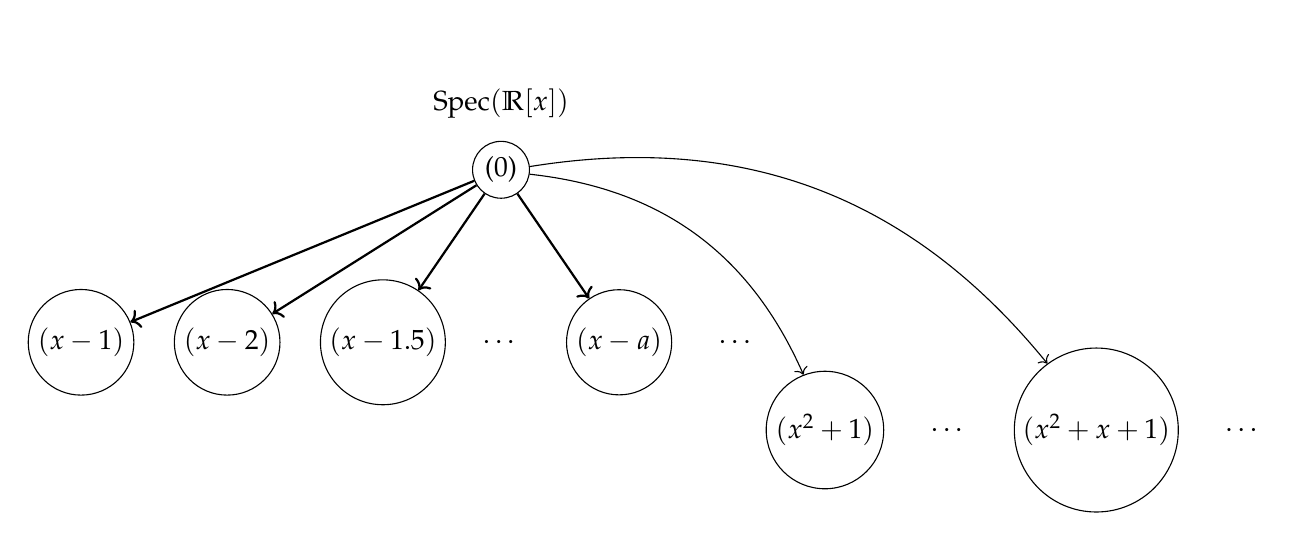
\begin{tikzpicture}[node distance=1.5cm, auto, every node/.style={draw, circle, inner sep=2pt}]
        % Generic point (0)
        \node (zero) {(0)};
        
        % Closed points for a few primes
        \node (dots) [below =of zero, draw=none] {$\dots$};
        \node (p) [right of= dots] {$(x-a)$};
        \node (dots2) [right of= p, draw=none] {$\dots$};

        \node (p5) [left of= dots] {$(x-1.5)$};
        \node (p3) [left =0.5of p5] {$(x-2)$};
        \node (p2) [left =0.5of p3] {$(x-1)$};

        
        \node (q1) [below right =0.5of dots2] {$(x^2+1)$};
        \node (qdots) [right =0.5of q1, draw=none] {$\dots$};
        \node (q2) [right =0.5of qdots] {$(x^2+x+1)$};
        \node (qdots2) [right =0.5of q2, draw=none] {$\dots$};
        
        % Arrows indicating specialization: (0) specializes to every maximal ideal.
        \draw[->, thick] (zero) -- (p2);
        \draw[->, thick] (zero) -- (p3);
        \draw[->, thick] (zero) -- (p5);
        \draw[->, thick] (zero) -- (p);
        \draw[->, bend left=30] (zero) to (q1);
        \draw[->, bend left=30] (zero) to (q2);

        \node[above=-0.5 of zero, align=center, draw=none] 
        {\(\operatorname{Spec}(\R[x])\)};
      \end{tikzpicture}

      \setcounter{enumi}{6}\item 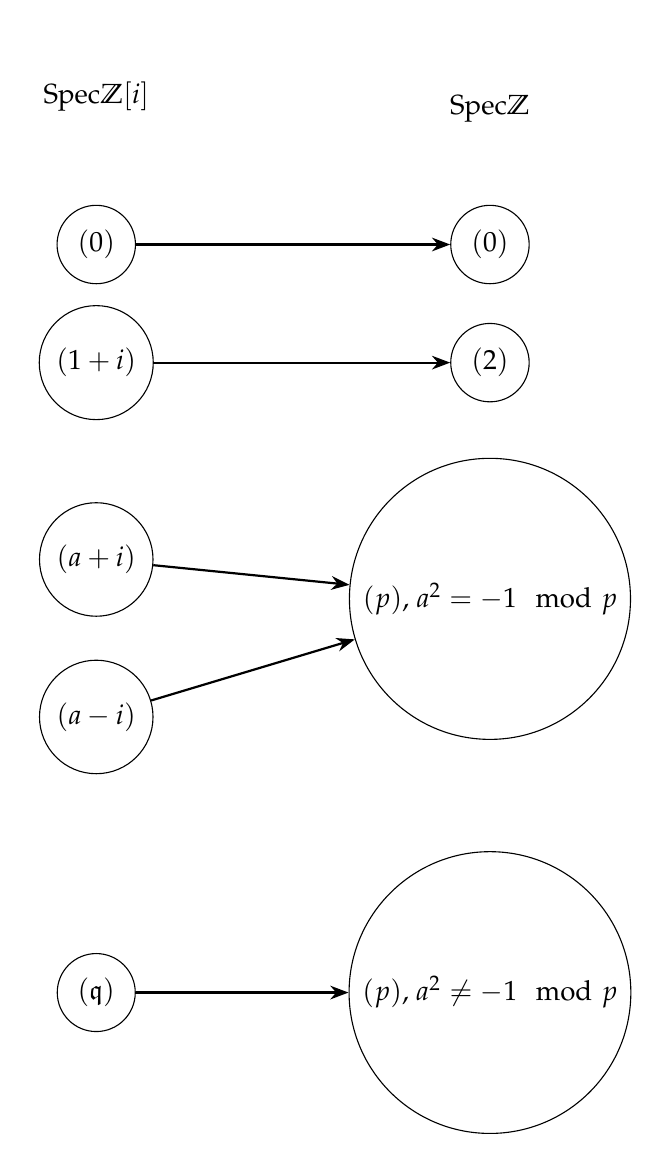
\begin{tikzpicture}[node distance=1.2cm and 1.5cm,
        every node/.style={draw, circle, inner sep=4pt},
        arrow/.style={->, >=Stealth, thick}]
      
        %%% Spec(Z[i]) column
        % Generic point in Spec(Z[i])
        \node (genZi) at (0,0) {$(0)$};
      
        % Ramified prime: (1+i) lying over 2.
        \node (ramZi) at (0,-1.5) {$(1+i)$};
      
        % Splitting prime: p ≡ 1 (mod 4) splits into two primes.
        \node (splitZi1) at (0,-4) {$(a+i)$};
        \node (splitZi2) at (0,-6) {$(a-i)$};
      
        % Inert prime: p ≡ 3 (mod 4)
        \node (inertZi) at (0,-9.5) {${(\mathfrak{q})}$};
      
        % Label the left column
        \node[above=0.5cm of genZi, draw=none] {Spec$\mathbb{Z}[i]$};
      
        %%% Spec(Z) column on the right
        % Generic point in Spec(Z)
        \node (genZ) at (5,0) {$(0)$};
        % The ideal (2)
        \node (p2Z) at (5,-1.5) {$(2)$};
        % The splitting prime image (same ideal for both primes over p)
        \node (pSplit) at (5,-4.5) {$(p)$, $a^2=-1 \mod p$};
        % The inert prime image
        \node (pInert) at (5,-9.5) {$(p)$, $a^2\neq-1 \mod p$};
      
        % Label the right column
        \node[above=0.5cm of genZ, draw=none] {Spec$\mathbb{Z}$};
      
        %%% Draw arrows to show the contraction of primes
        \draw[arrow] (genZi) -- (genZ);
        \draw[arrow] (ramZi) -- (p2Z);
        \draw[arrow] (splitZi1) -- (pSplit);
        \draw[arrow] (splitZi2) -- (pSplit);
        \draw[arrow] (inertZi) -- (pInert);
      \end{tikzpicture}
 \end{enumerate}
\end{document}